%% Default Latex document template
%%
%%  blake@rcs.ee.washington.edu

\documentclass[letterpaper]{article}

% Uncomment for bibliog.
%\bibliographystyle{unsrt}

\usepackage{graphicx}
\usepackage{lineno}
%\usepackage{fancyhdr}

%%%%%%%%%%%%%%%%%%%%%%%%%%%%%%%%%%%%%%%%5
%
%  Set Up Margins
\input{templates/pagedim.tex}

%
%        Font selection
%
%\renewcommand{\rmdefault}{ptm}             % Times
%\renewcommand{\rmdefault}{phv}             % Helvetica
%\renewcommand{\rmdefault}{pcr}             % Courier
%\renewcommand{\rmdefault}{pbk}             % Bookman
%\renewcommand{\rmdefault}{pag}             % Avant Garde
%\renewcommand{\rmdefault}{ppl}             % Palatino
%\renewcommand{\rmdefault}{pch}             % Charter


%%%%%%%%%%%%%%%%%%%%%%%%%%%%%%%%%%%%%%%%%%%%%%%%%
%
%         Page format Mods HERE
%
%Mod's to page size for this document
\addtolength\textwidth{0cm}
\addtolength\oddsidemargin{0cm}
\addtolength\headsep{0cm}
\addtolength\textheight{0cm}
%\linespread{0.894}   % 0.894 = 6 lines per inch, 1 = "single",  1.6 = "double"

% header options for fancyhdr

%\pagestyle{fancy}
%\lhead{LEFT HEADER}
%\chead{CENTER HEADER}
%\rhead{RIGHT HEADER}
%\lfoot{Hannaford, U. of Washington}
%\rfoot{\today}
%\cfoot{\thepage}



% Make table rows deeper
%\renewcommand\arraystretch{2.0}% Vertical Row size, 1.0 is for standard spacing)

\begin{document}
\section*{Path Optimization: Brute Force Search}

\section{Basics}

\subsection{Notation}
The goal is to search a grid of points in the  space consisting of points  $P_i = \{X_i, V_i\} = \{x,y,z,\dot{x},\dot{y},\dot{z}\}$ within bounds:
\[
-1 < x < 1, \;
-1 < y < 1, \;
-1 < z < 1, \;
-1 < \dot{x} < 1, \;
-1 < \dot{y} < 1, \;
-1 < \dot{z} < 1, \;
\]

occuring within a time $\Delta t$.    We wish to visit all the points with as low a cost as possible.

We have $N$ points per axis, for a total of $6^N$ points.

A {\it trajectory}, $T_{ij}$ between two points in this space, $T(P_i,P_j)$, is a route through
the space from $P_i$ to $P_{i+1}$ with the properties

\beq \label{firstconstraint}
\Delta X (T_{ij}) = \frac{X_{i+1}-X_i}{\Delta t}
\eeq

\beq
| \frac {\Delta V} {\Delta t} |_\infty  < a_{max}
\eeq
\beq
| \frac {\Delta V} {\Delta t} |_\infty < v_{max}
\eeq
\beq \label{complexconstraint}\label{lastconstraint}
|\Delta V +  \frac {\Delta X}{\Delta t} |_\infty < v_{max}
\eeq

\begin{figure}\centering
  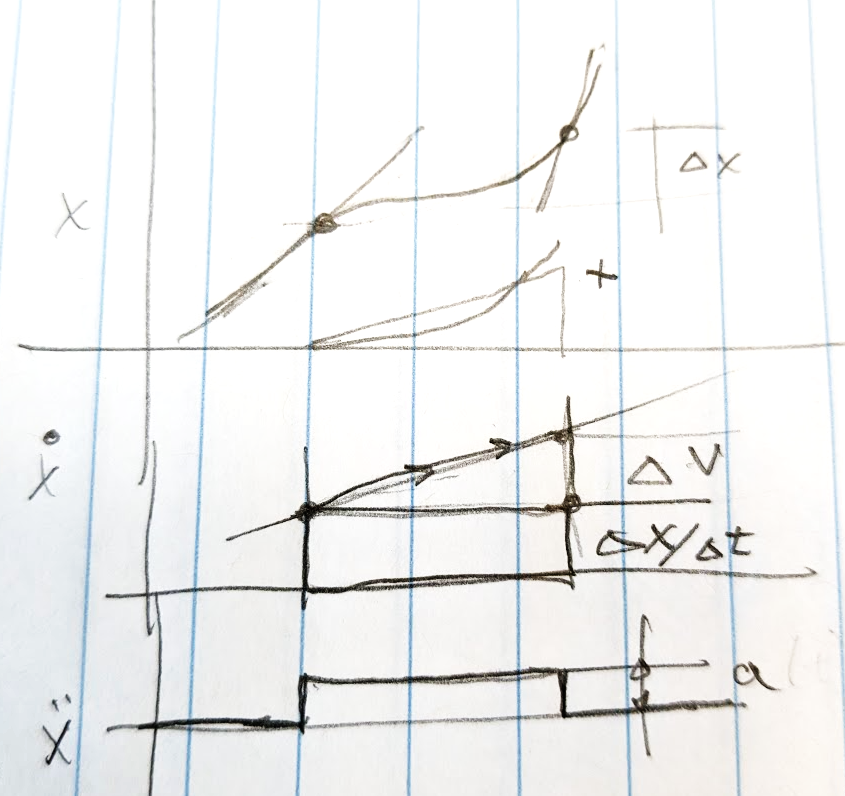
\includegraphics[width=3.0in]{basicTraj.png}
  \caption{}\label{basicTraj}
\end{figure}
Constraint eqn (\ref{complexconstraint}) can be seen from Figure \ref{basicTraj}.   Two components of ${V}_i$
are shown, one arising from $\Delta X$ and another arising from $\Delta V$.

Assuming we let $|a| = a_{max}$ then
\beq
\Delta t = \frac{\Delta V}{a_{max}}
\eeq\label{deltat}

\subsection{Trajectory Cost}
Our goal is to find a minimum cost trajectory and we can define the cost of a trajectory at least two ways:

\subsubsection{Energy Cost}    We assume that energy of a trajectory is proportional to acceleration times time.  Give our assumption
of eqn(\ref{deltat}, the energy cost, $C_e$, is
\beq
C_{e}(T_{ij}) = |a_{max}\Delta t| = |\Delta V|
\eeq

\subsubsection{Duration Cost}   The time cost, $C_t$ is
\beq
C_t(T_{ij}) = \Delta t
\eeq

\subsection{Path Cost}
A {\it path}, $\mathbf{P}$, is an ordered sequence of the points $P_i$ covering the entire grid.
Let $C_i$ be the cost of the trajectory from $P_i$ to $P_{i+1}$ where the $P_i$ belong to $\mathbf{P}$.
The time   cost of visiting every point with a given path is
\beq
C_T = \Sigma_i C_i  \qquad 0 \leq i < 6^N
\eeq
For example, the total duration cost of path $\mathbf{P}_1$ would be
\beq
C_{Td} = \Sigma_i C_t(T_{ij})
\eeq
where $T_{ij}$ is the $i^{th}$ trajectory of $\mathbf{P}_1$ defined by $T(P_i, P_j)$.

\section{Problem Statement}

We can now state our problem as, given a set of points defining a uniform grid in a position and velocity
space, with $N$ points between bounds $\{-1,1\}$ in each dimension, find the path $\mathbf{P}_{opt}$
that visits all the points with the lowest overall cost.   This problem is similar to the famous
Traveling Salesman problem, but the map is simplified by a grid patterns and our coordinates are coupled by
the fact that
\beq
X(t) = \int_0^t V(t) dt
\eeq
Because of the constraints (eqns \ref{firstconstraint} to \ref{lastconstraint}), this reduces to
choosing the sequence of points visited.


\section{Brute force searching}

\subsection{1D example}
We start with a simple case of a two dimensional space consisting of a scalar position and velocity.  We grid the
space with $N=4$ points in position and velocity for a total of 16 points.

Some possible trajectories are shown in Figure \ref{handsolutions1D}.


\begin{figure}\centering
  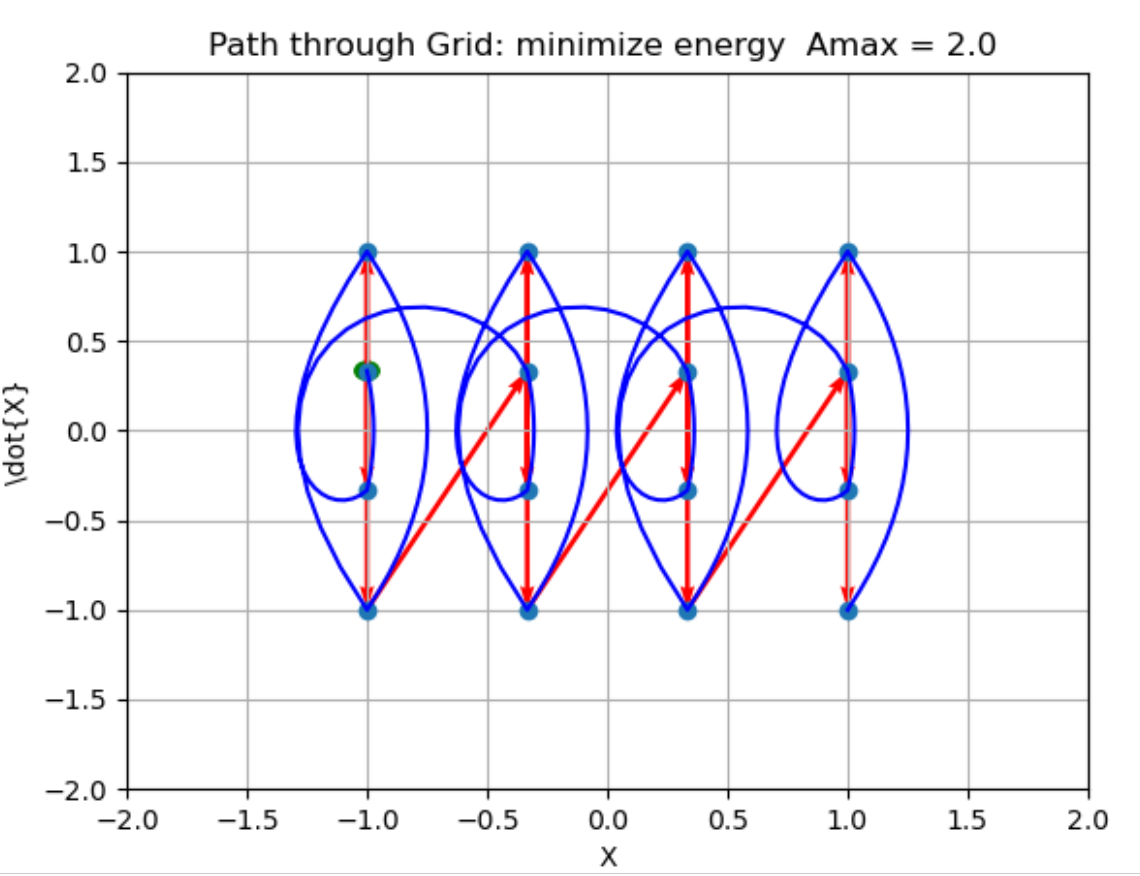
\includegraphics[width=3.0in]{handTraj01.png}
  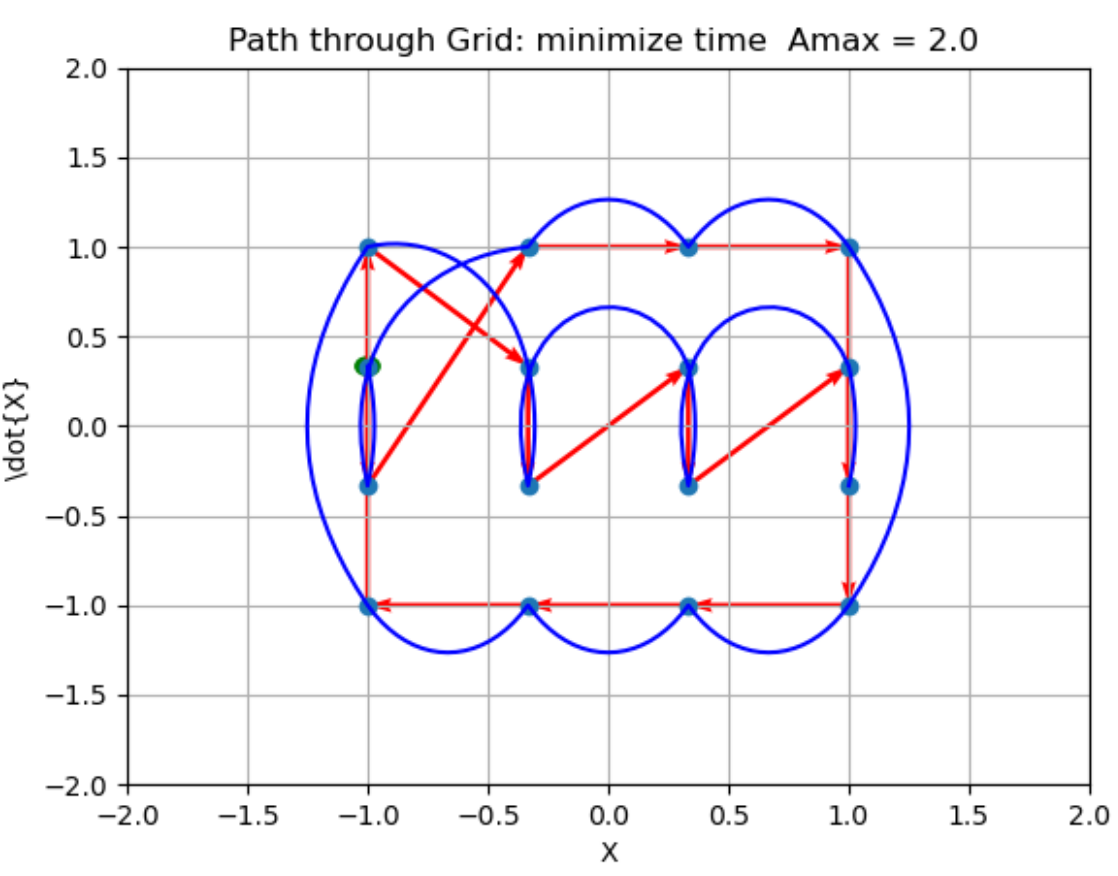
\includegraphics[width=3.0in]{handTraj02.png}
  \caption{}\label{handsolutions1D}
\end{figure}

The first one appears economical but it cannot visit the line $\dot{x} = 0$.  The second one may be plausible,
but is it optimal?   Does it extend ``too far" beyond the boundaries?

Also, logically the starting point should be on the zero velocity line, but this requires a diagonal start.

\subsection{simulation structure}
We define the following classes:
\begin{itemize}
  \item {\tt grid}   The grid and associated methods.
  \item {\tt point}  A single point and associated methods.
  \item {\tt trajectory} A trajectory between two points and methods for time-evolution, cost computation.
\end{itemize}

\subsection{overall strategy}

\begin{enumerate}
  \item Create the grid and associated points
  \item Compute for each point, compute the cost of a trajectory between it and all the other points.  Populate
  a cost matrix with $N^6$ rows and $N^6$ columns where
  \beq
    Cm_{ij} = C_x(T_{ij})  \qquad    x \in \{e,t\}
  \eeq
  \item Manually select starting point ($P_0$)
  \item Select the lowest cost column from the starting point row of $Cm$.
  \item Block that point (marking a list)
  \item Repeat until all points are blocked.
\end{enumerate}

\end{document}

